\color{red}\huge{TODO metti il nome in inglese}\color{black}
\section{creaFoglioRiepilogativo}
\centering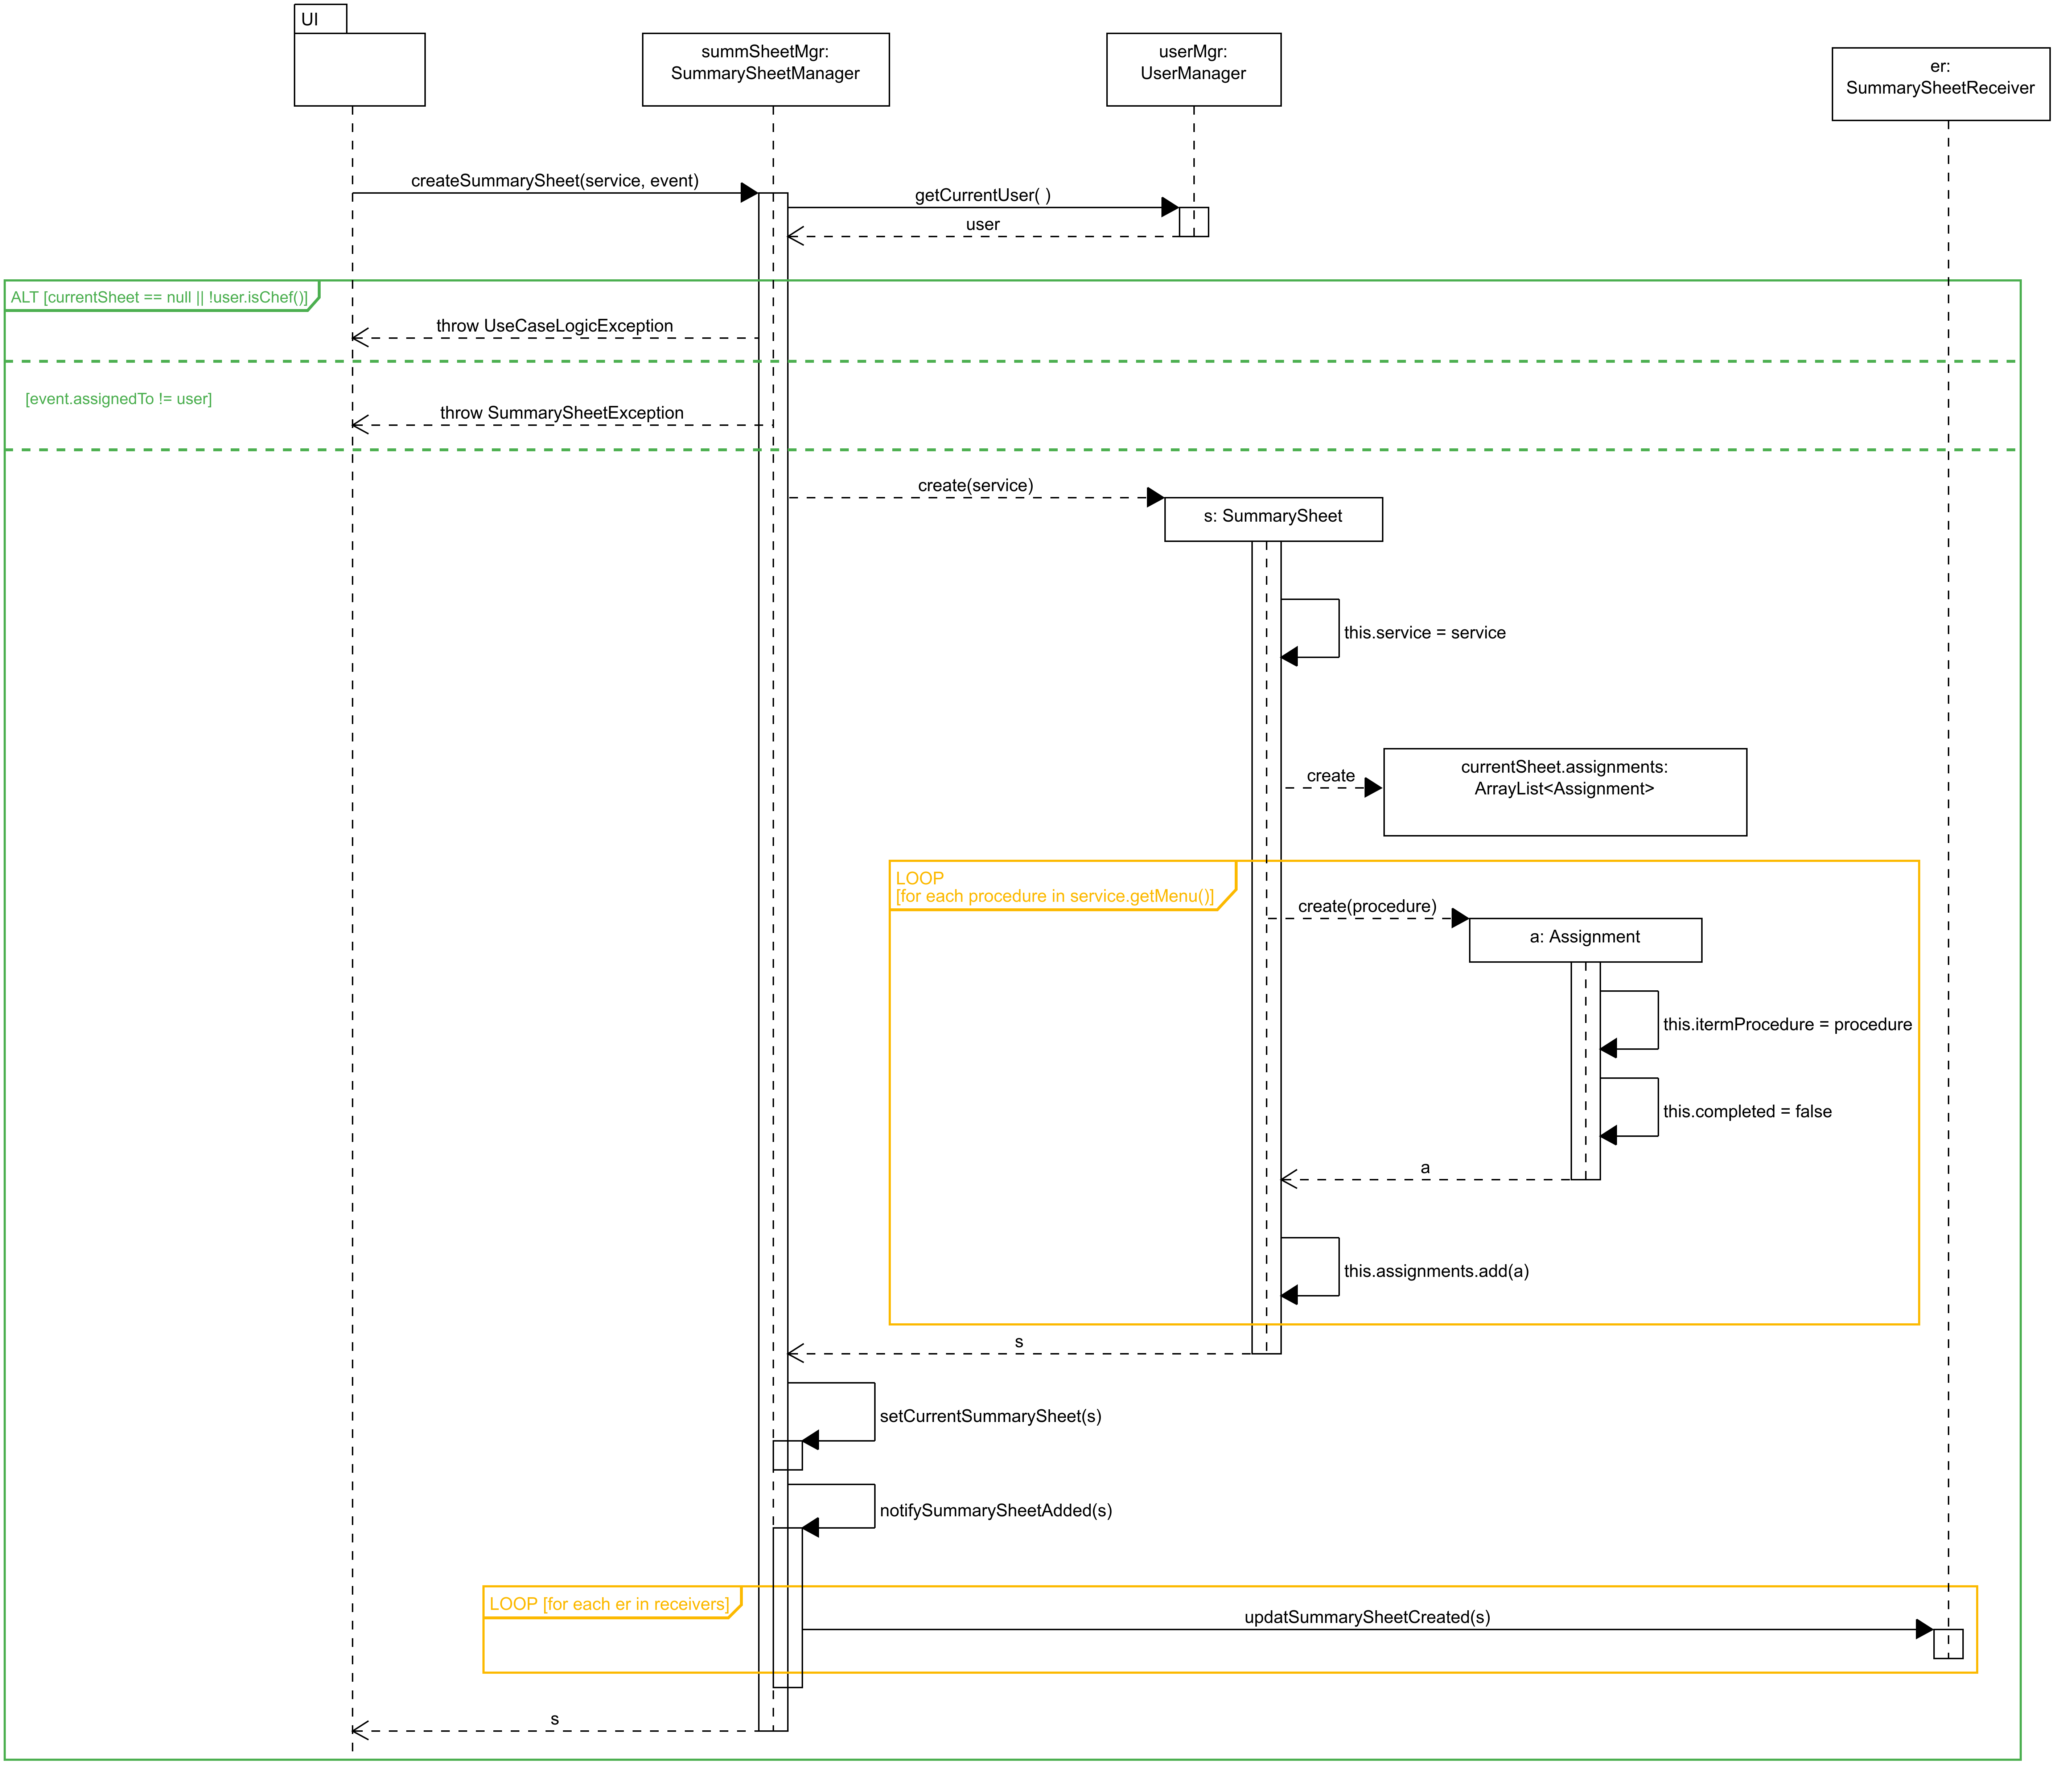
\includegraphics[max width=\textwidth, max height=158mm]{../resources/img/GCC/DSD/op1.png}

\subsection{scegliFoglioRiepilogativo}
\centering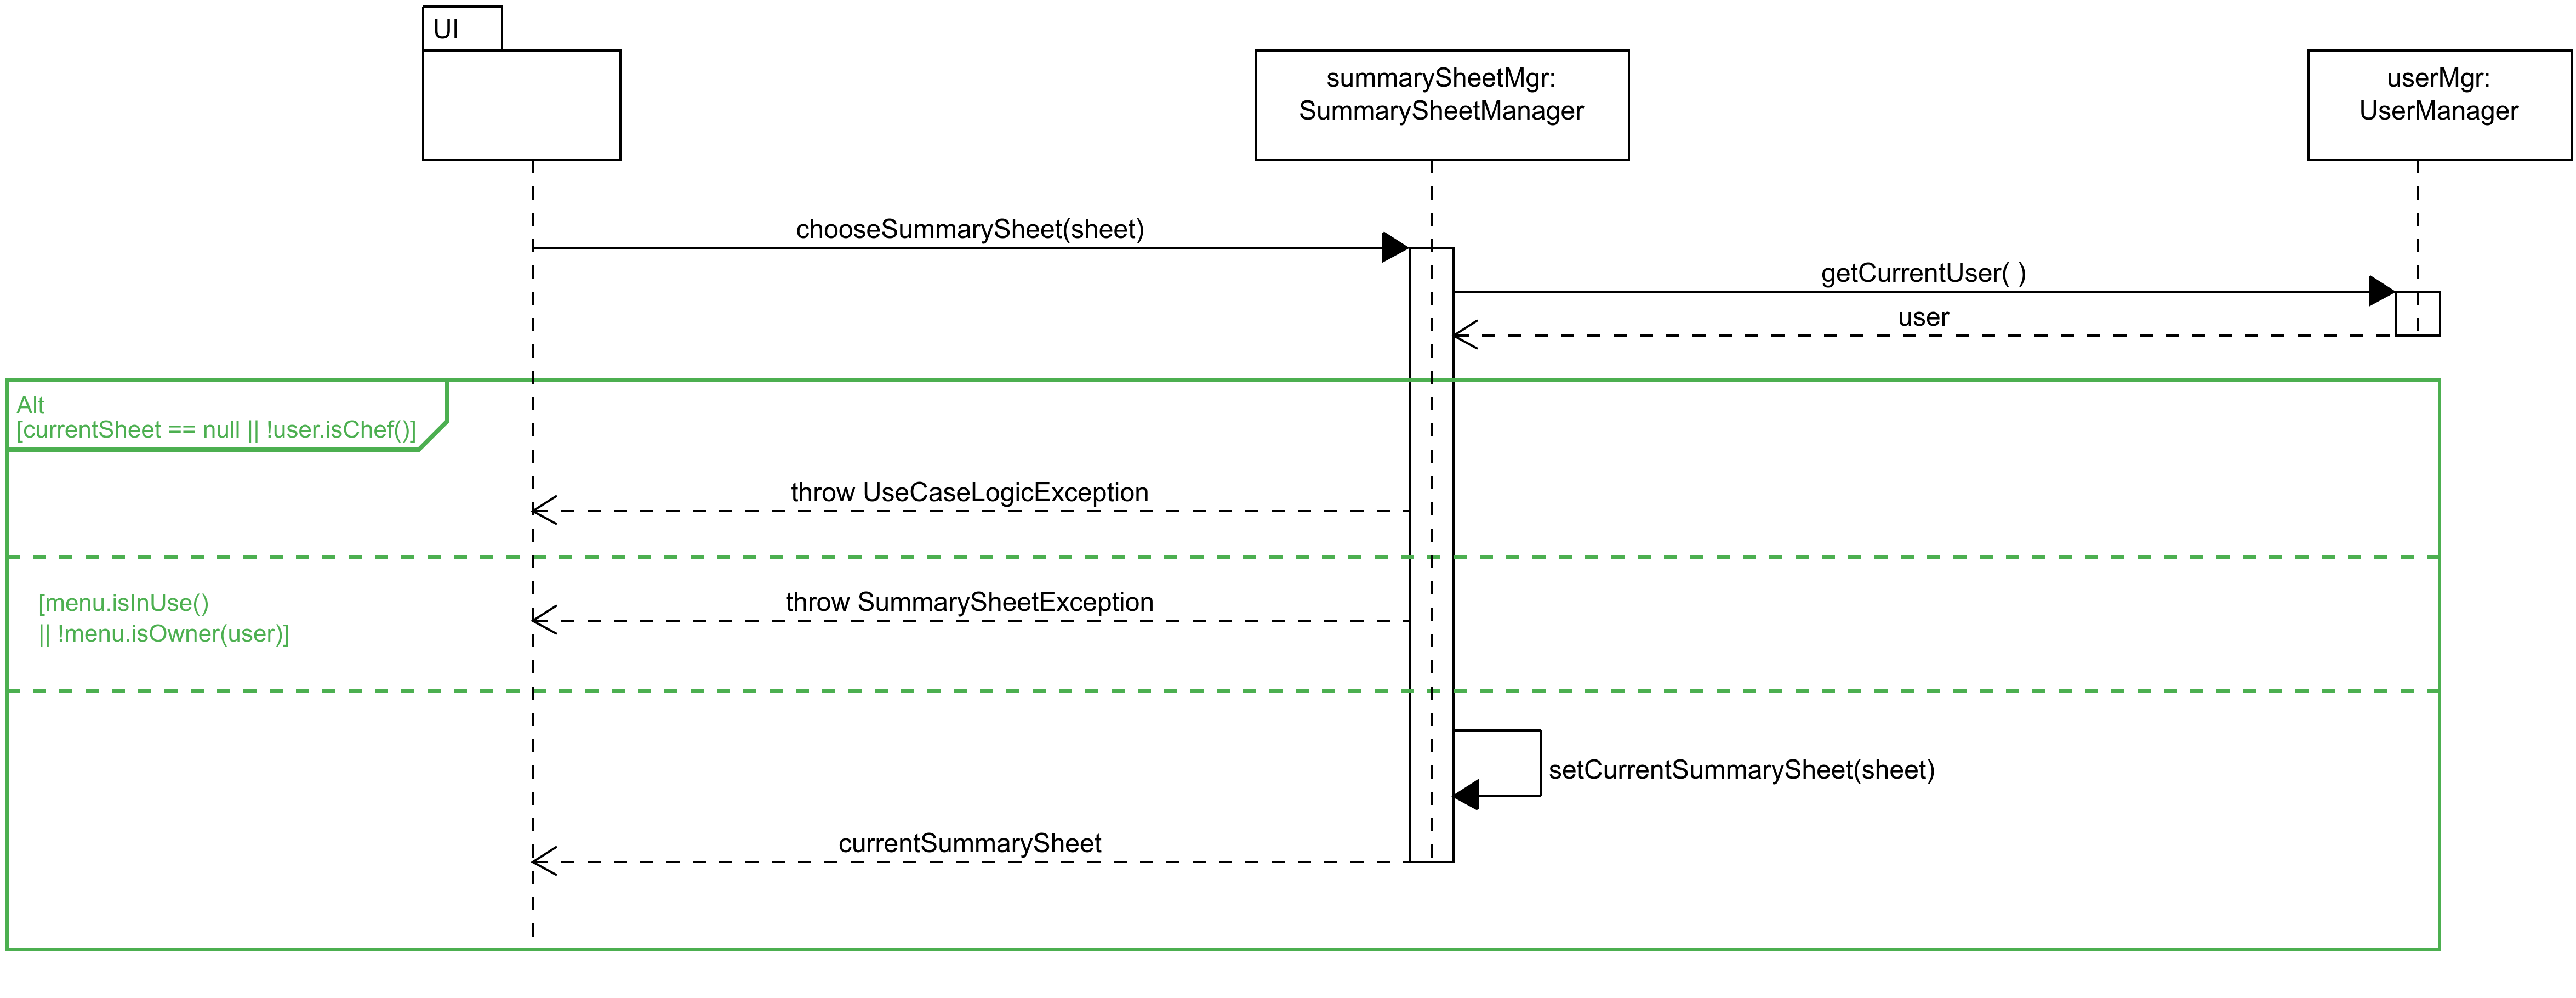
\includegraphics[max width=\textwidth, max height=190mm]{../resources/img/GCC/DSD/op1a.png}

\section{aggiungiProcedura}
\centering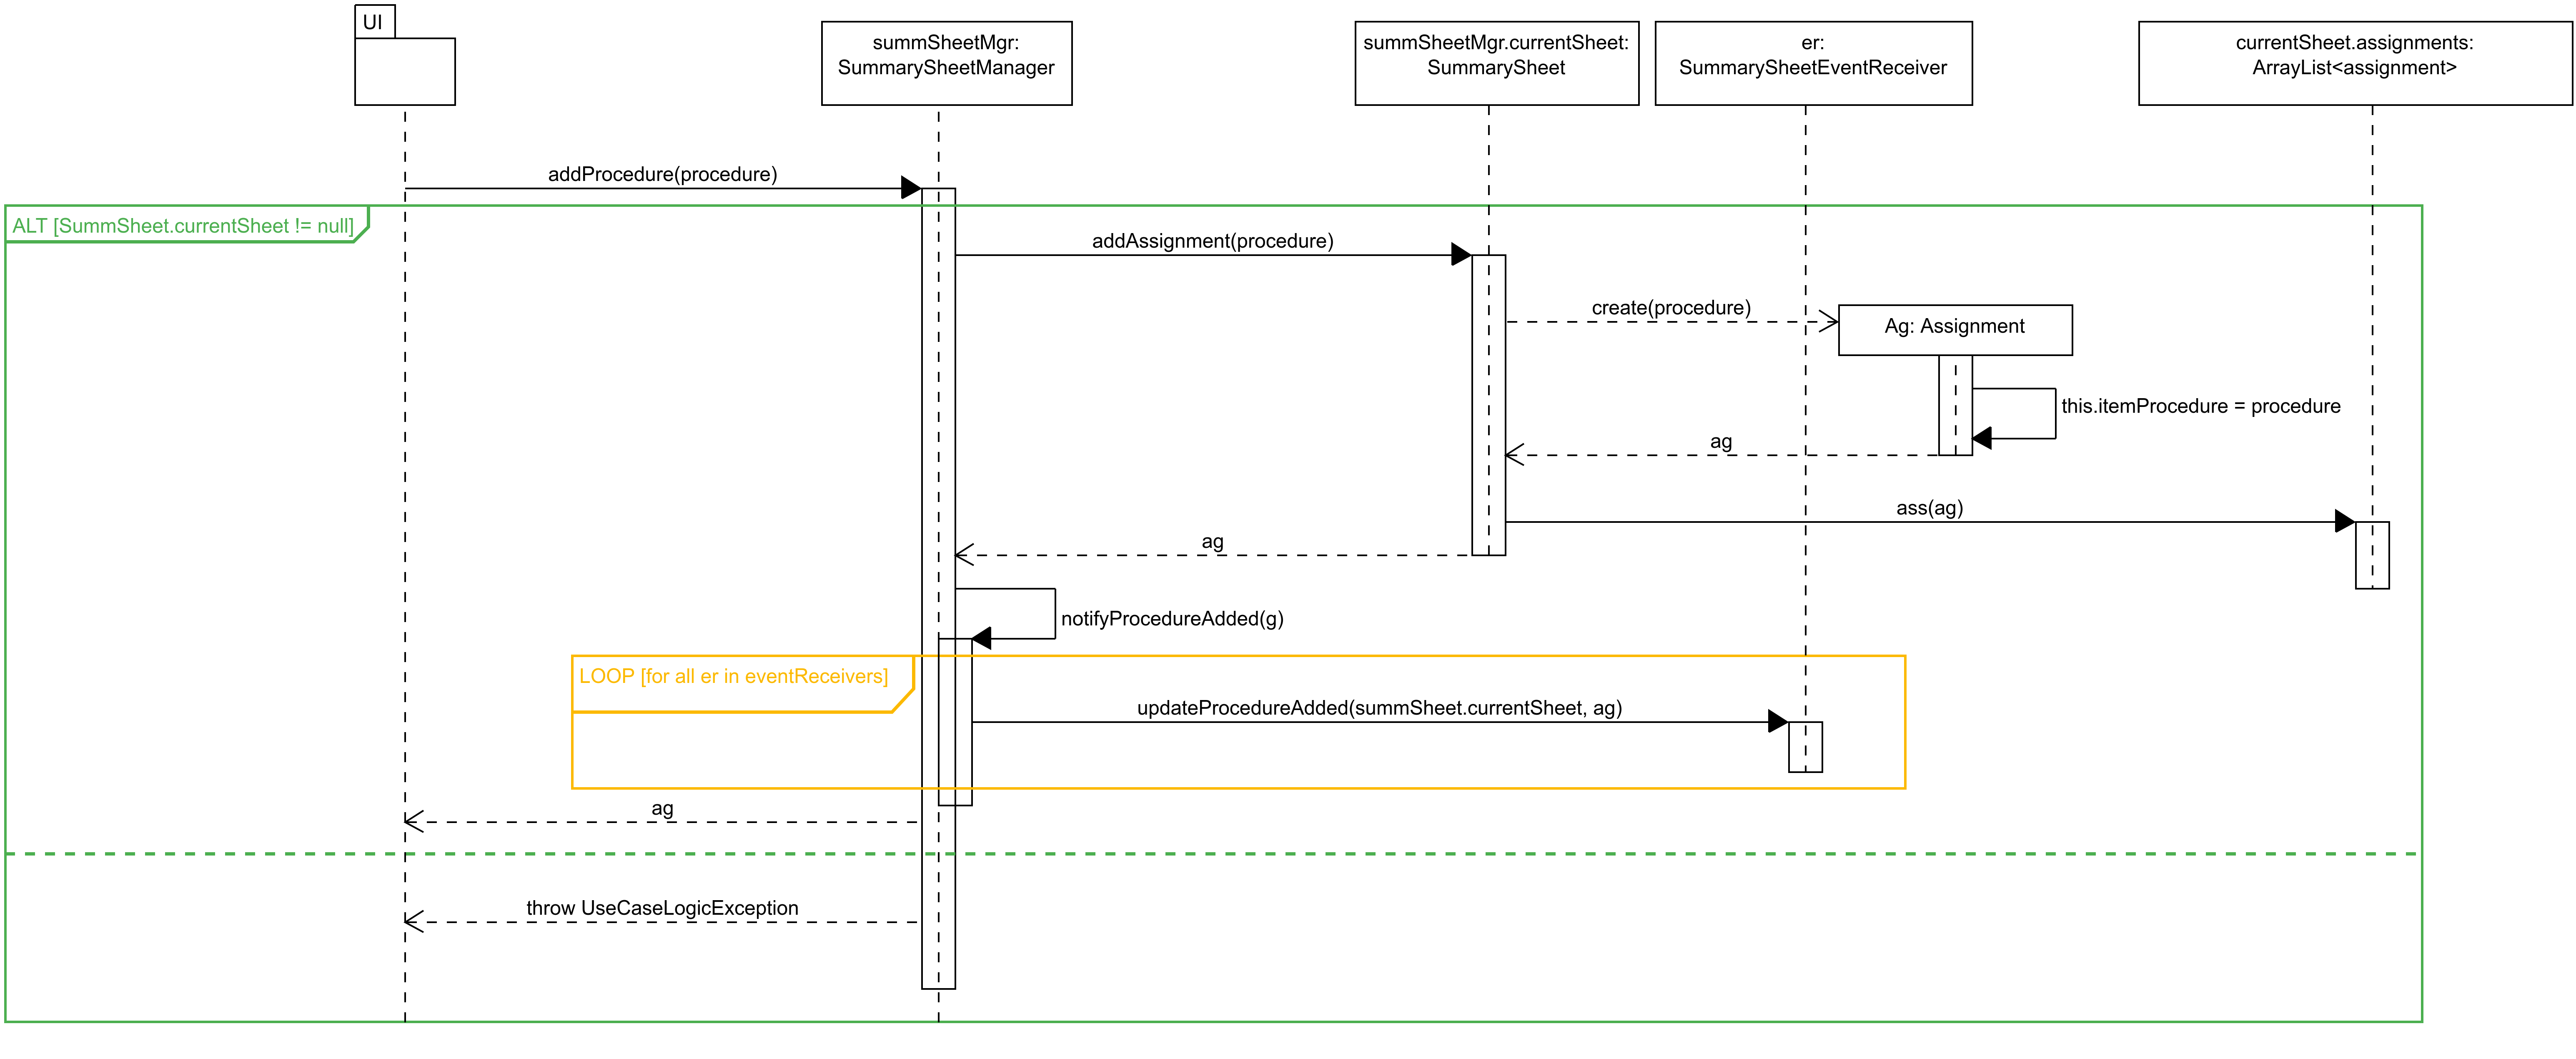
\includegraphics[max width=\textwidth, max height=190mm]{../resources/img/GCC/DSD/op2.png}

\subsection{eliminaProcedura}
\centering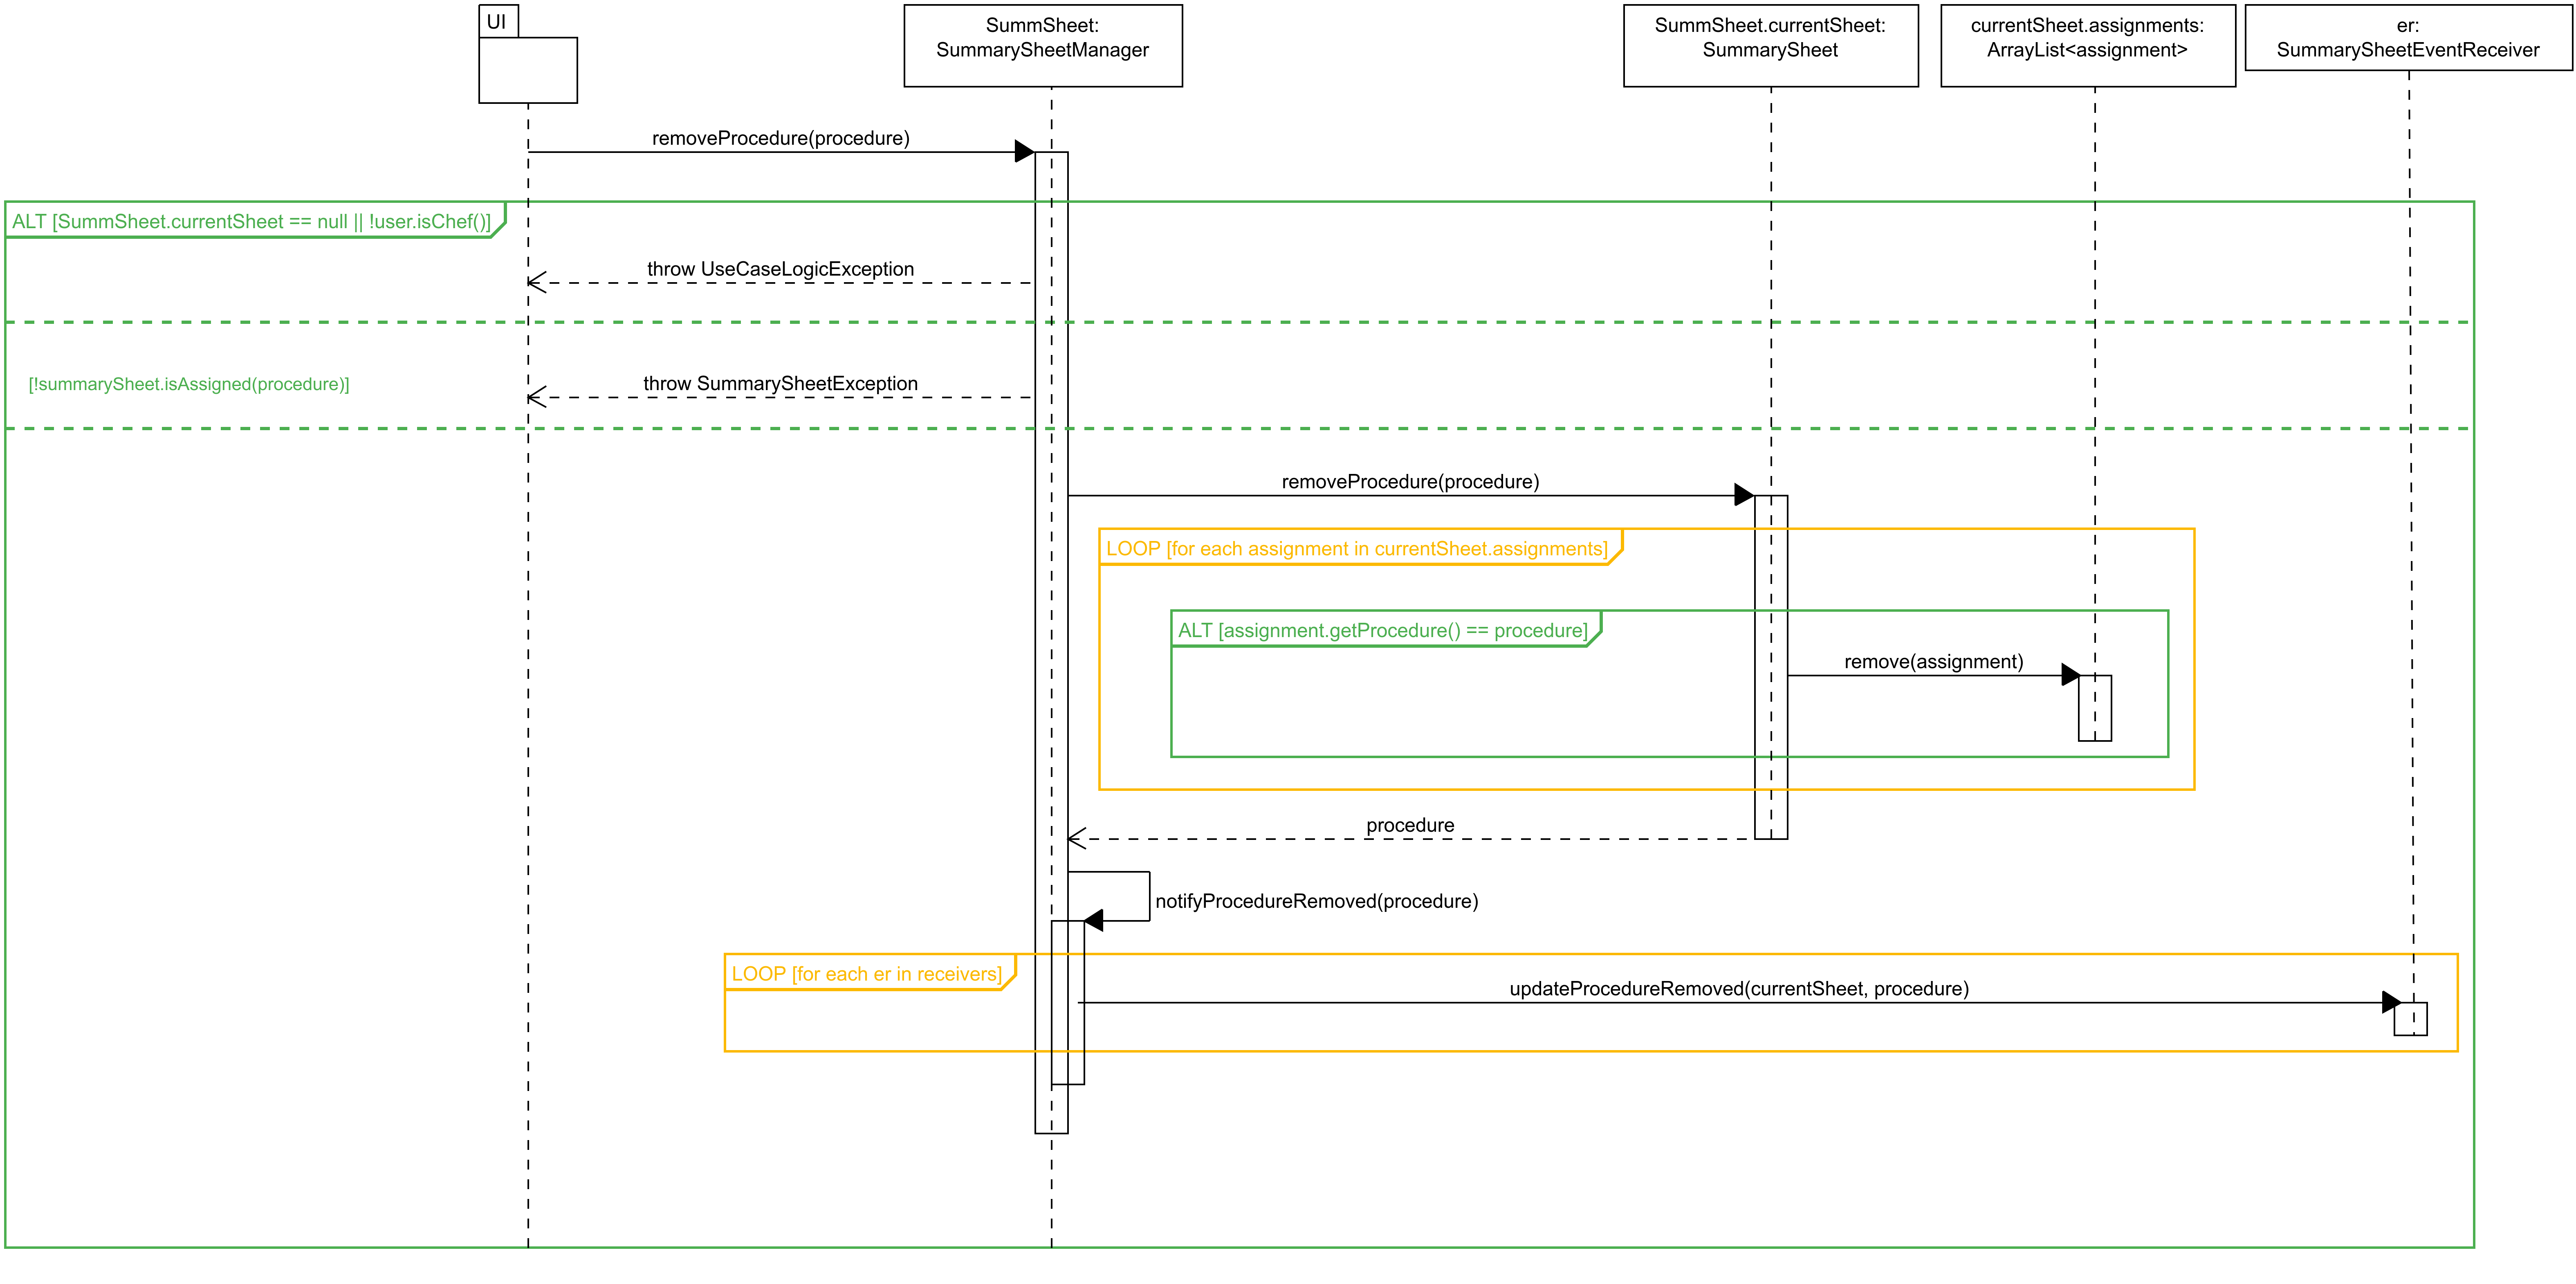
\includegraphics[max width=\textwidth, max height=190mm]{../resources/img/GCC/DSD/op2a.png}

\section{riordinaElencoAssegnamenti}
\centering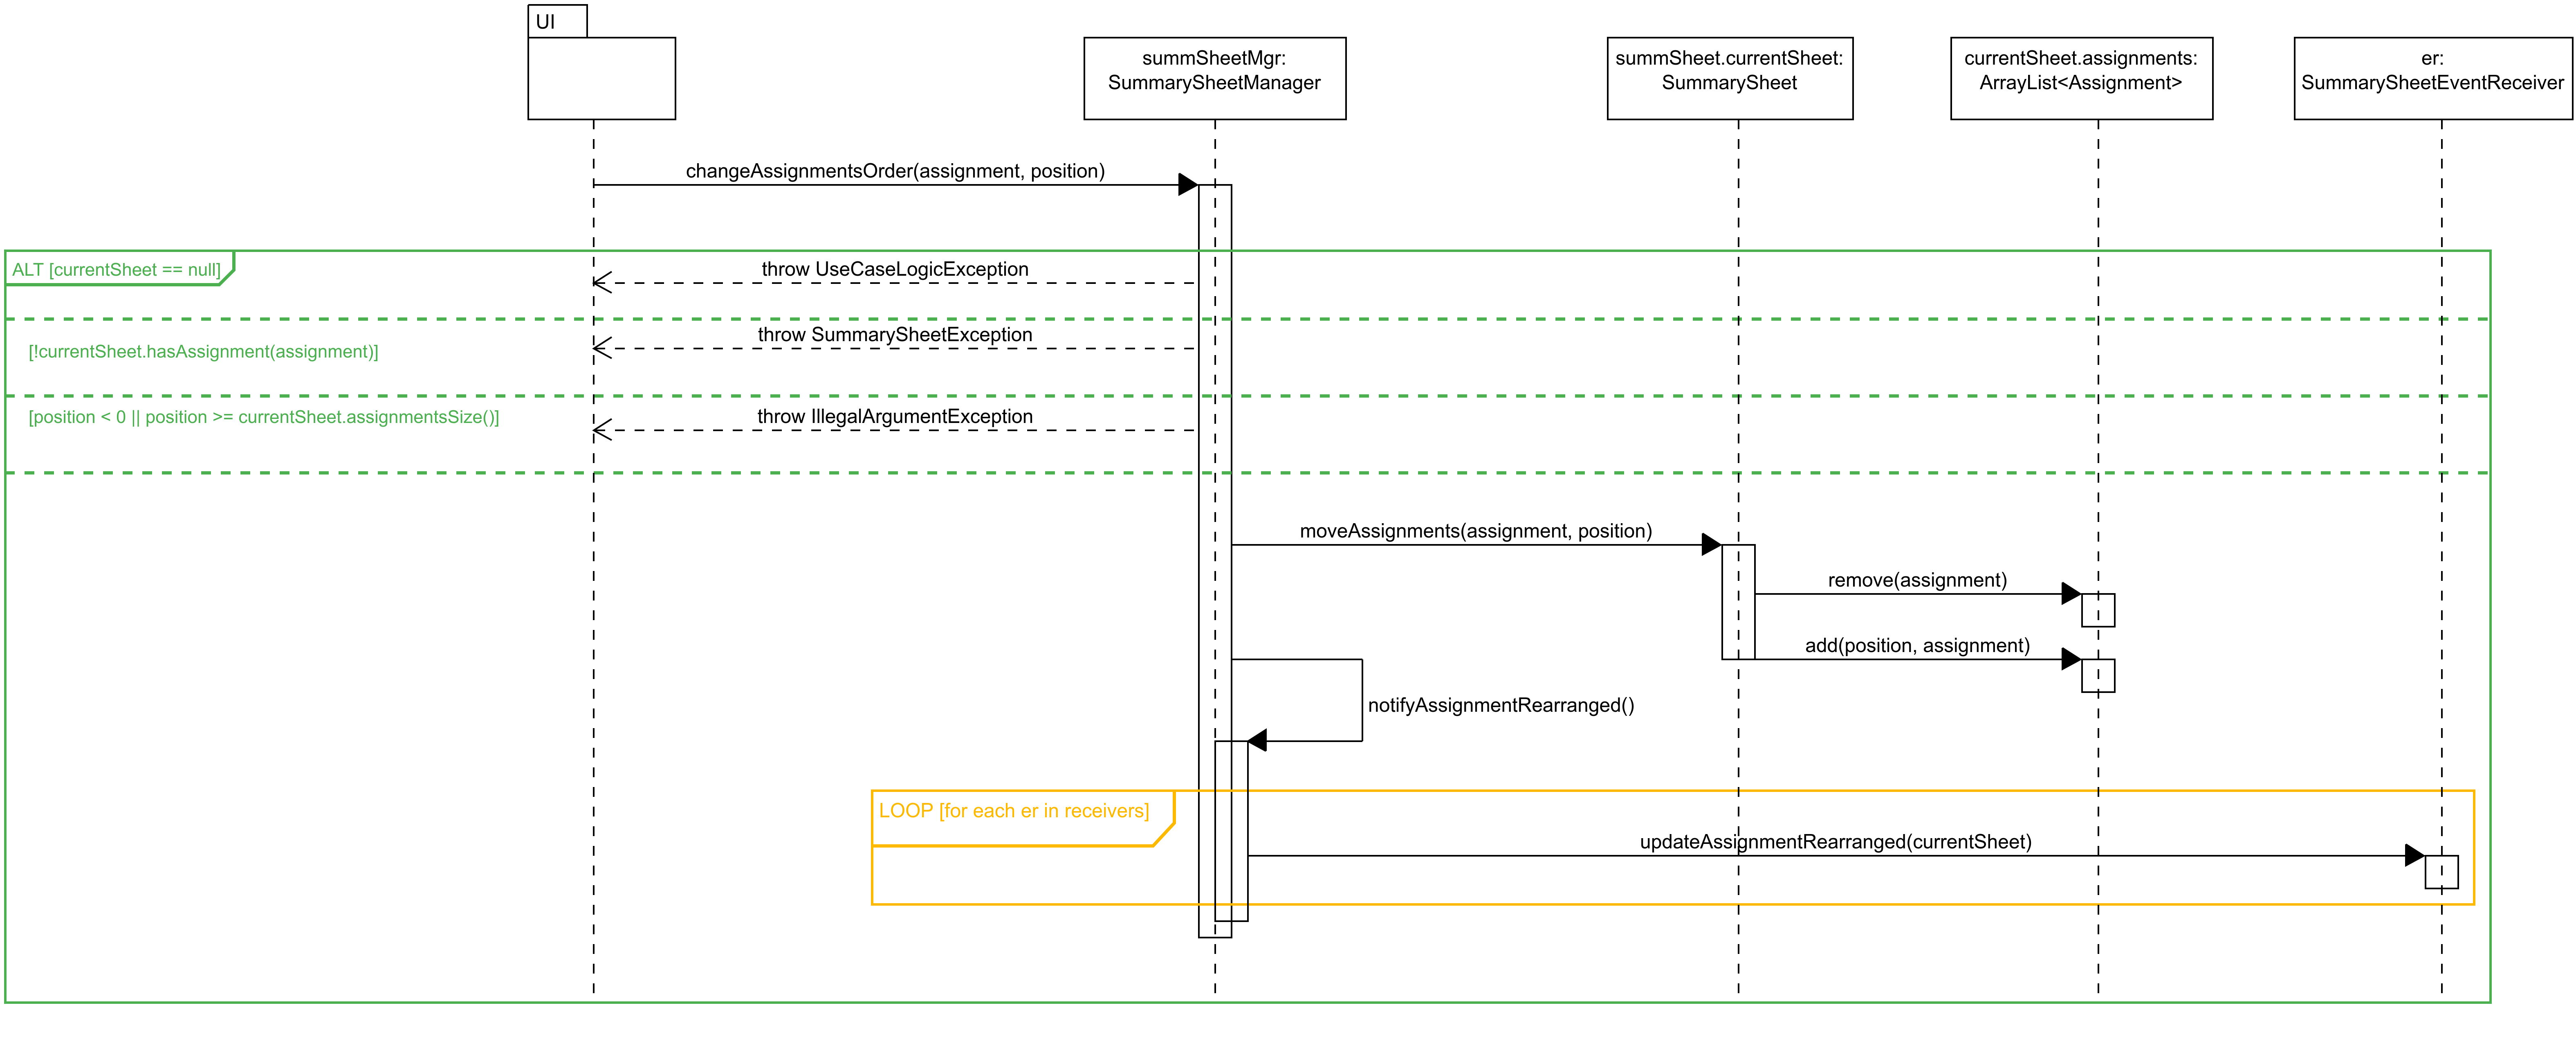
\includegraphics[max width=\textwidth, max height=190mm]{../resources/img/GCC/DSD/op3.png}

\section{consultaTabelloneTurni}
\centering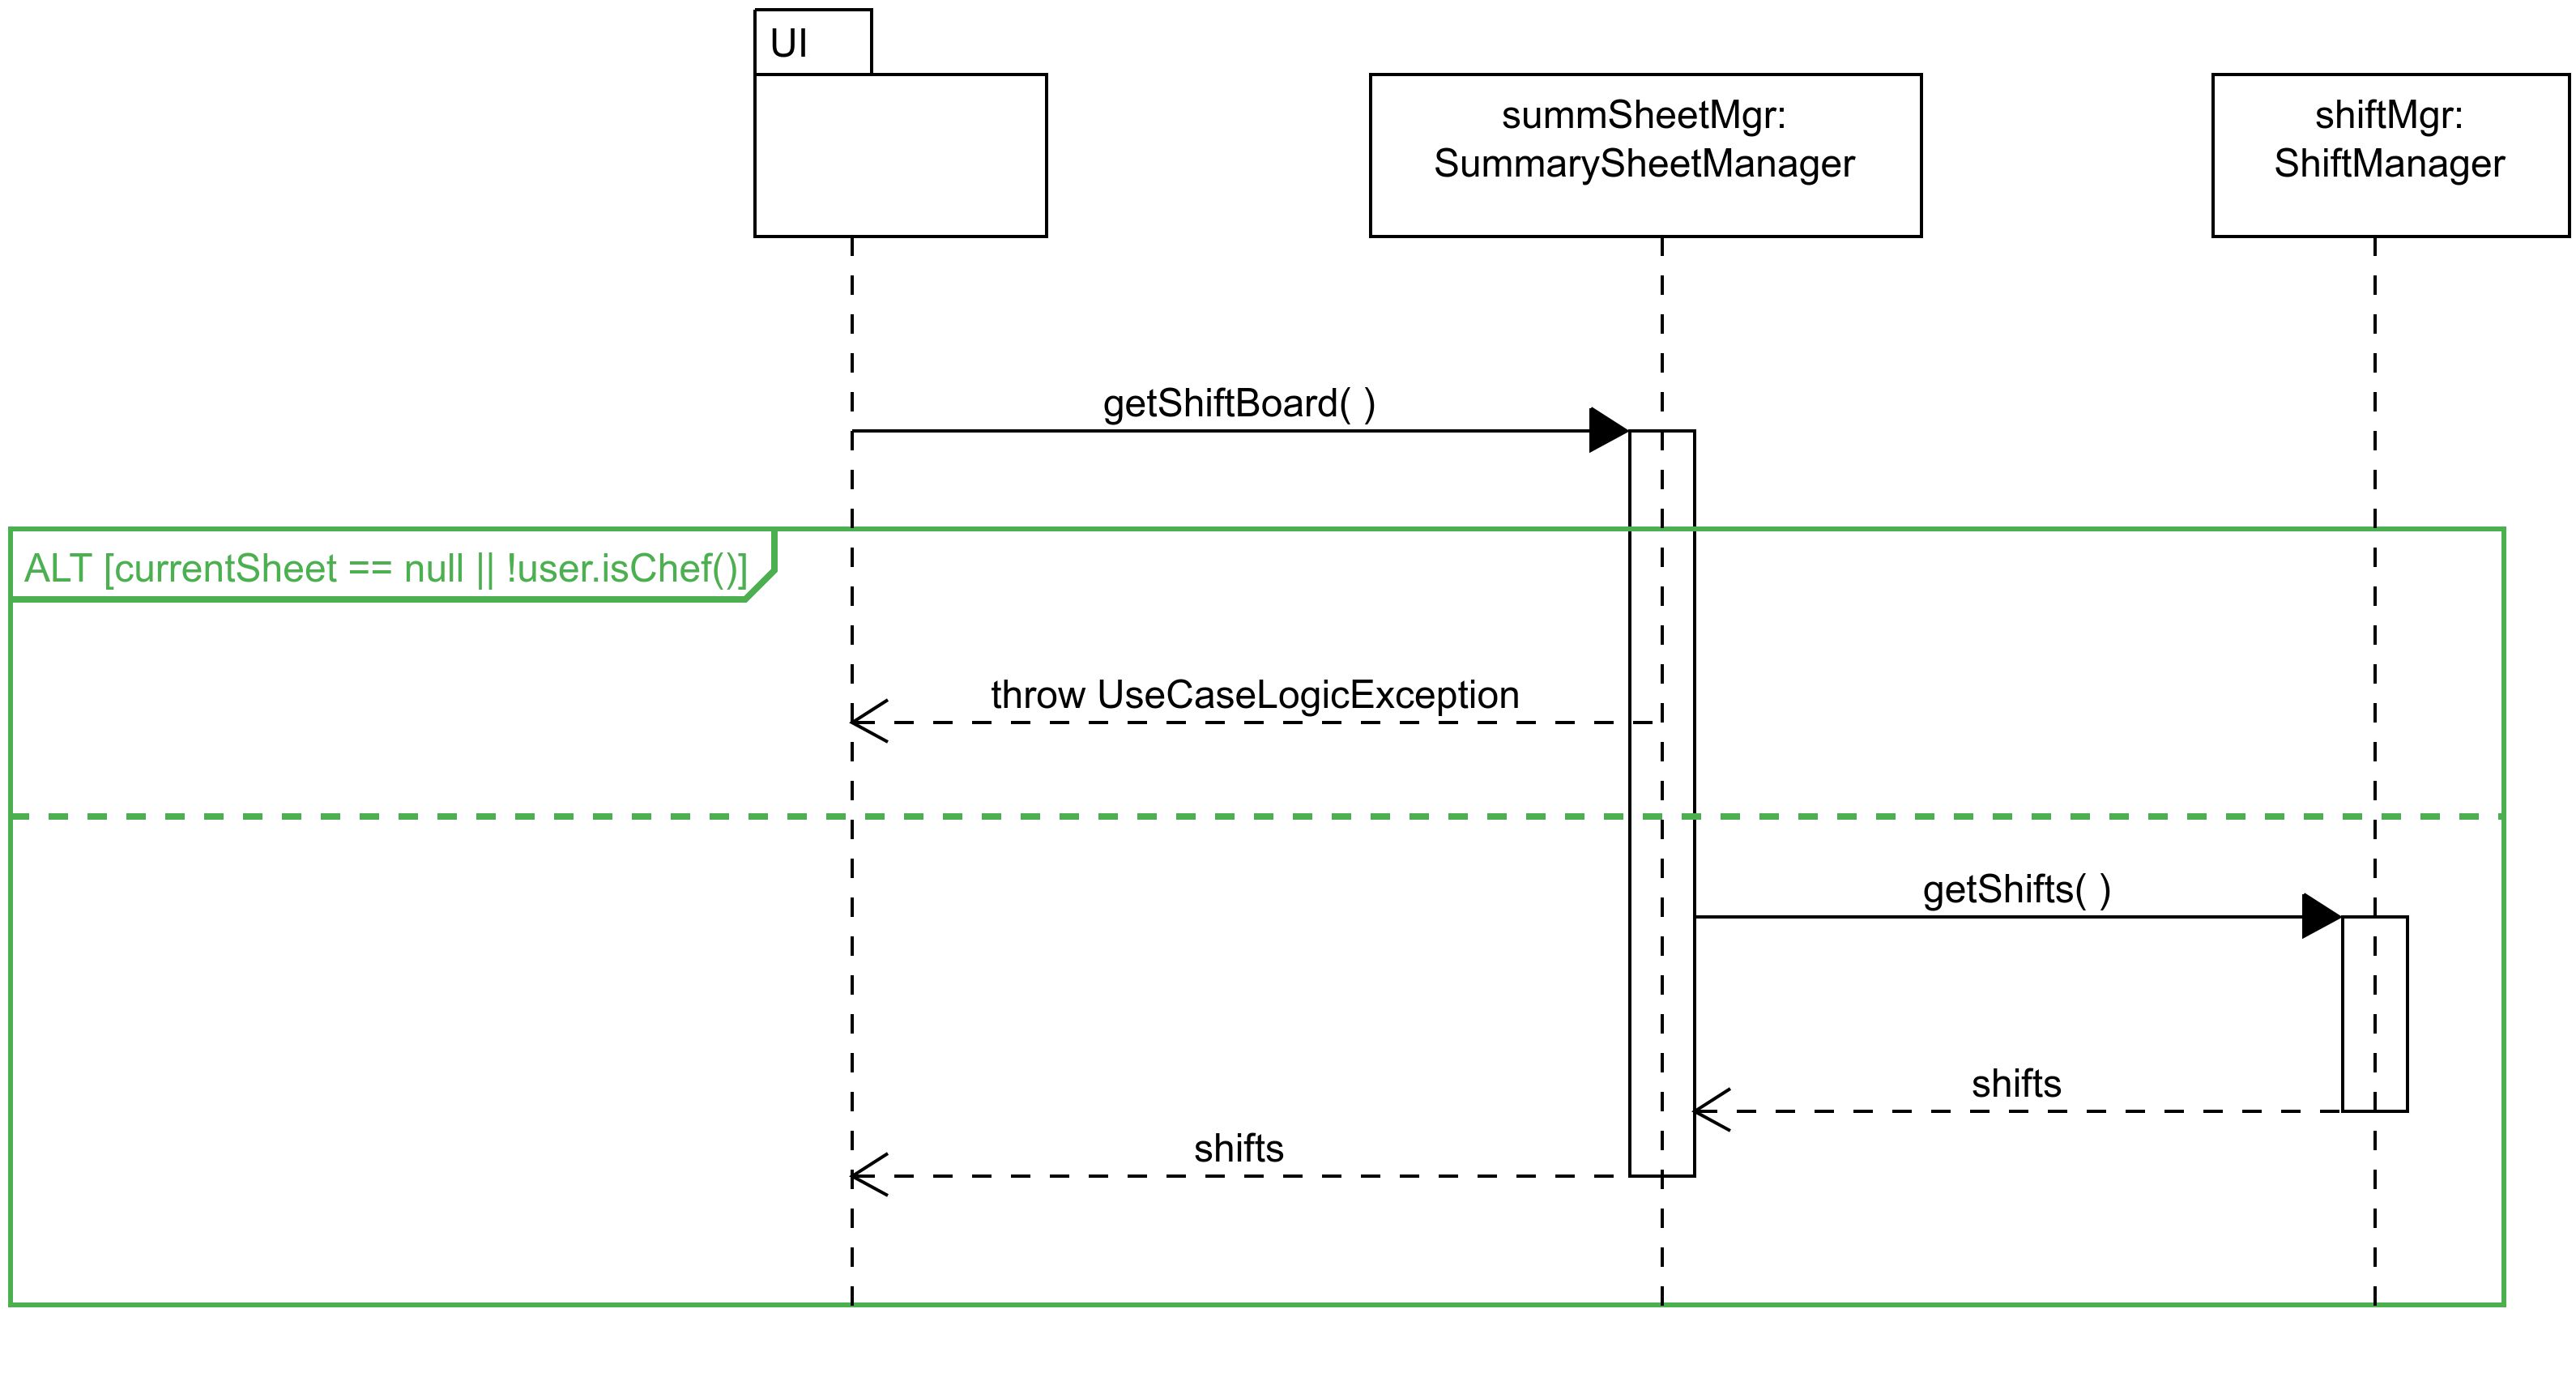
\includegraphics[max width=\textwidth, max height=190mm]{../resources/img/GCC/DSD/op4.png}

\section{generaAssegnamento}
\centering\includegraphics[max width=\textwidth, max height=190mm]{../resources/img/GCC/DSD/op5.png}

\subsection{specificaAssegnamentoCompletato}
\centering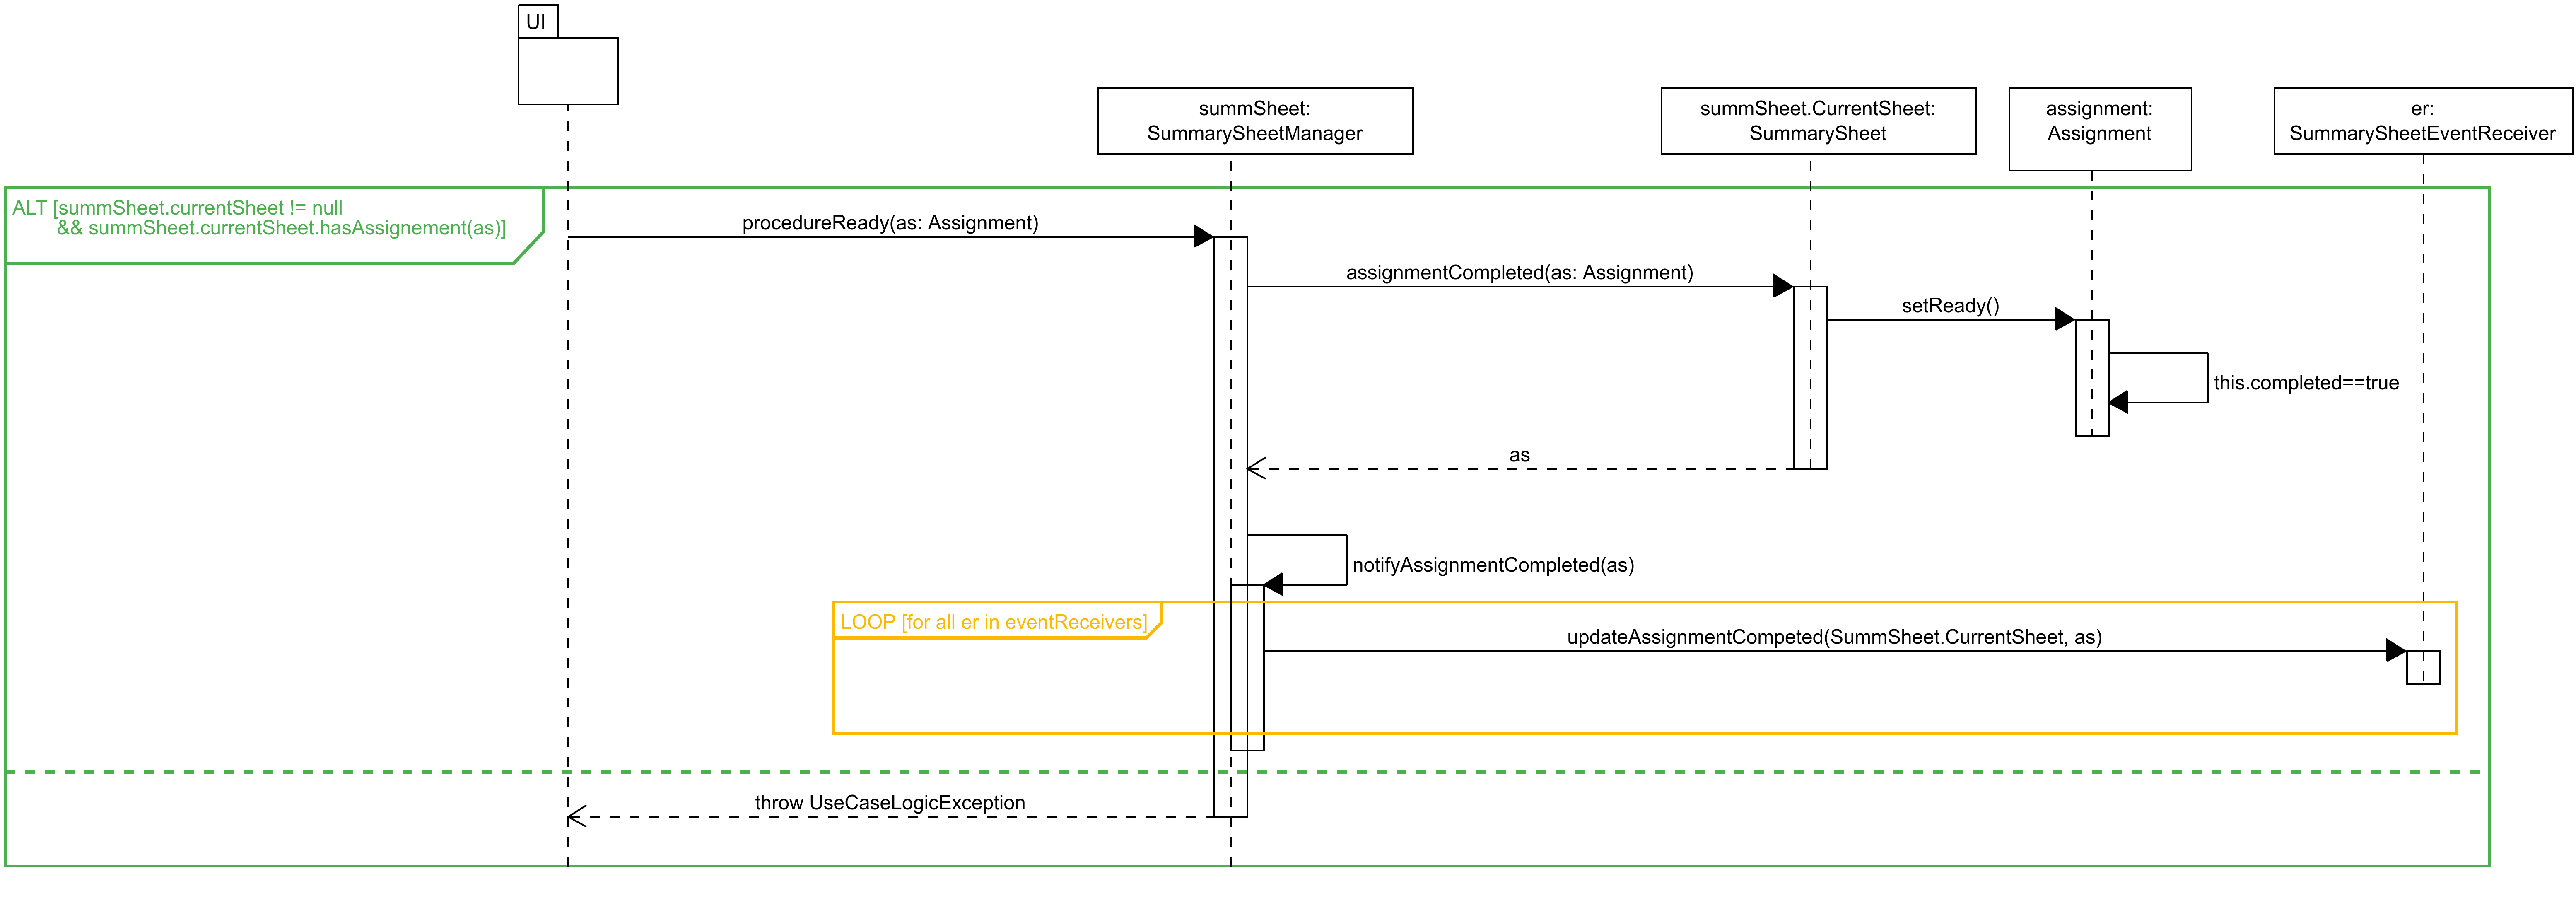
\includegraphics[max width=\textwidth, max height=190mm]{../resources/img/GCC/DSD/op5a.png}

\subsection{eliminaAssegnamento}
\centering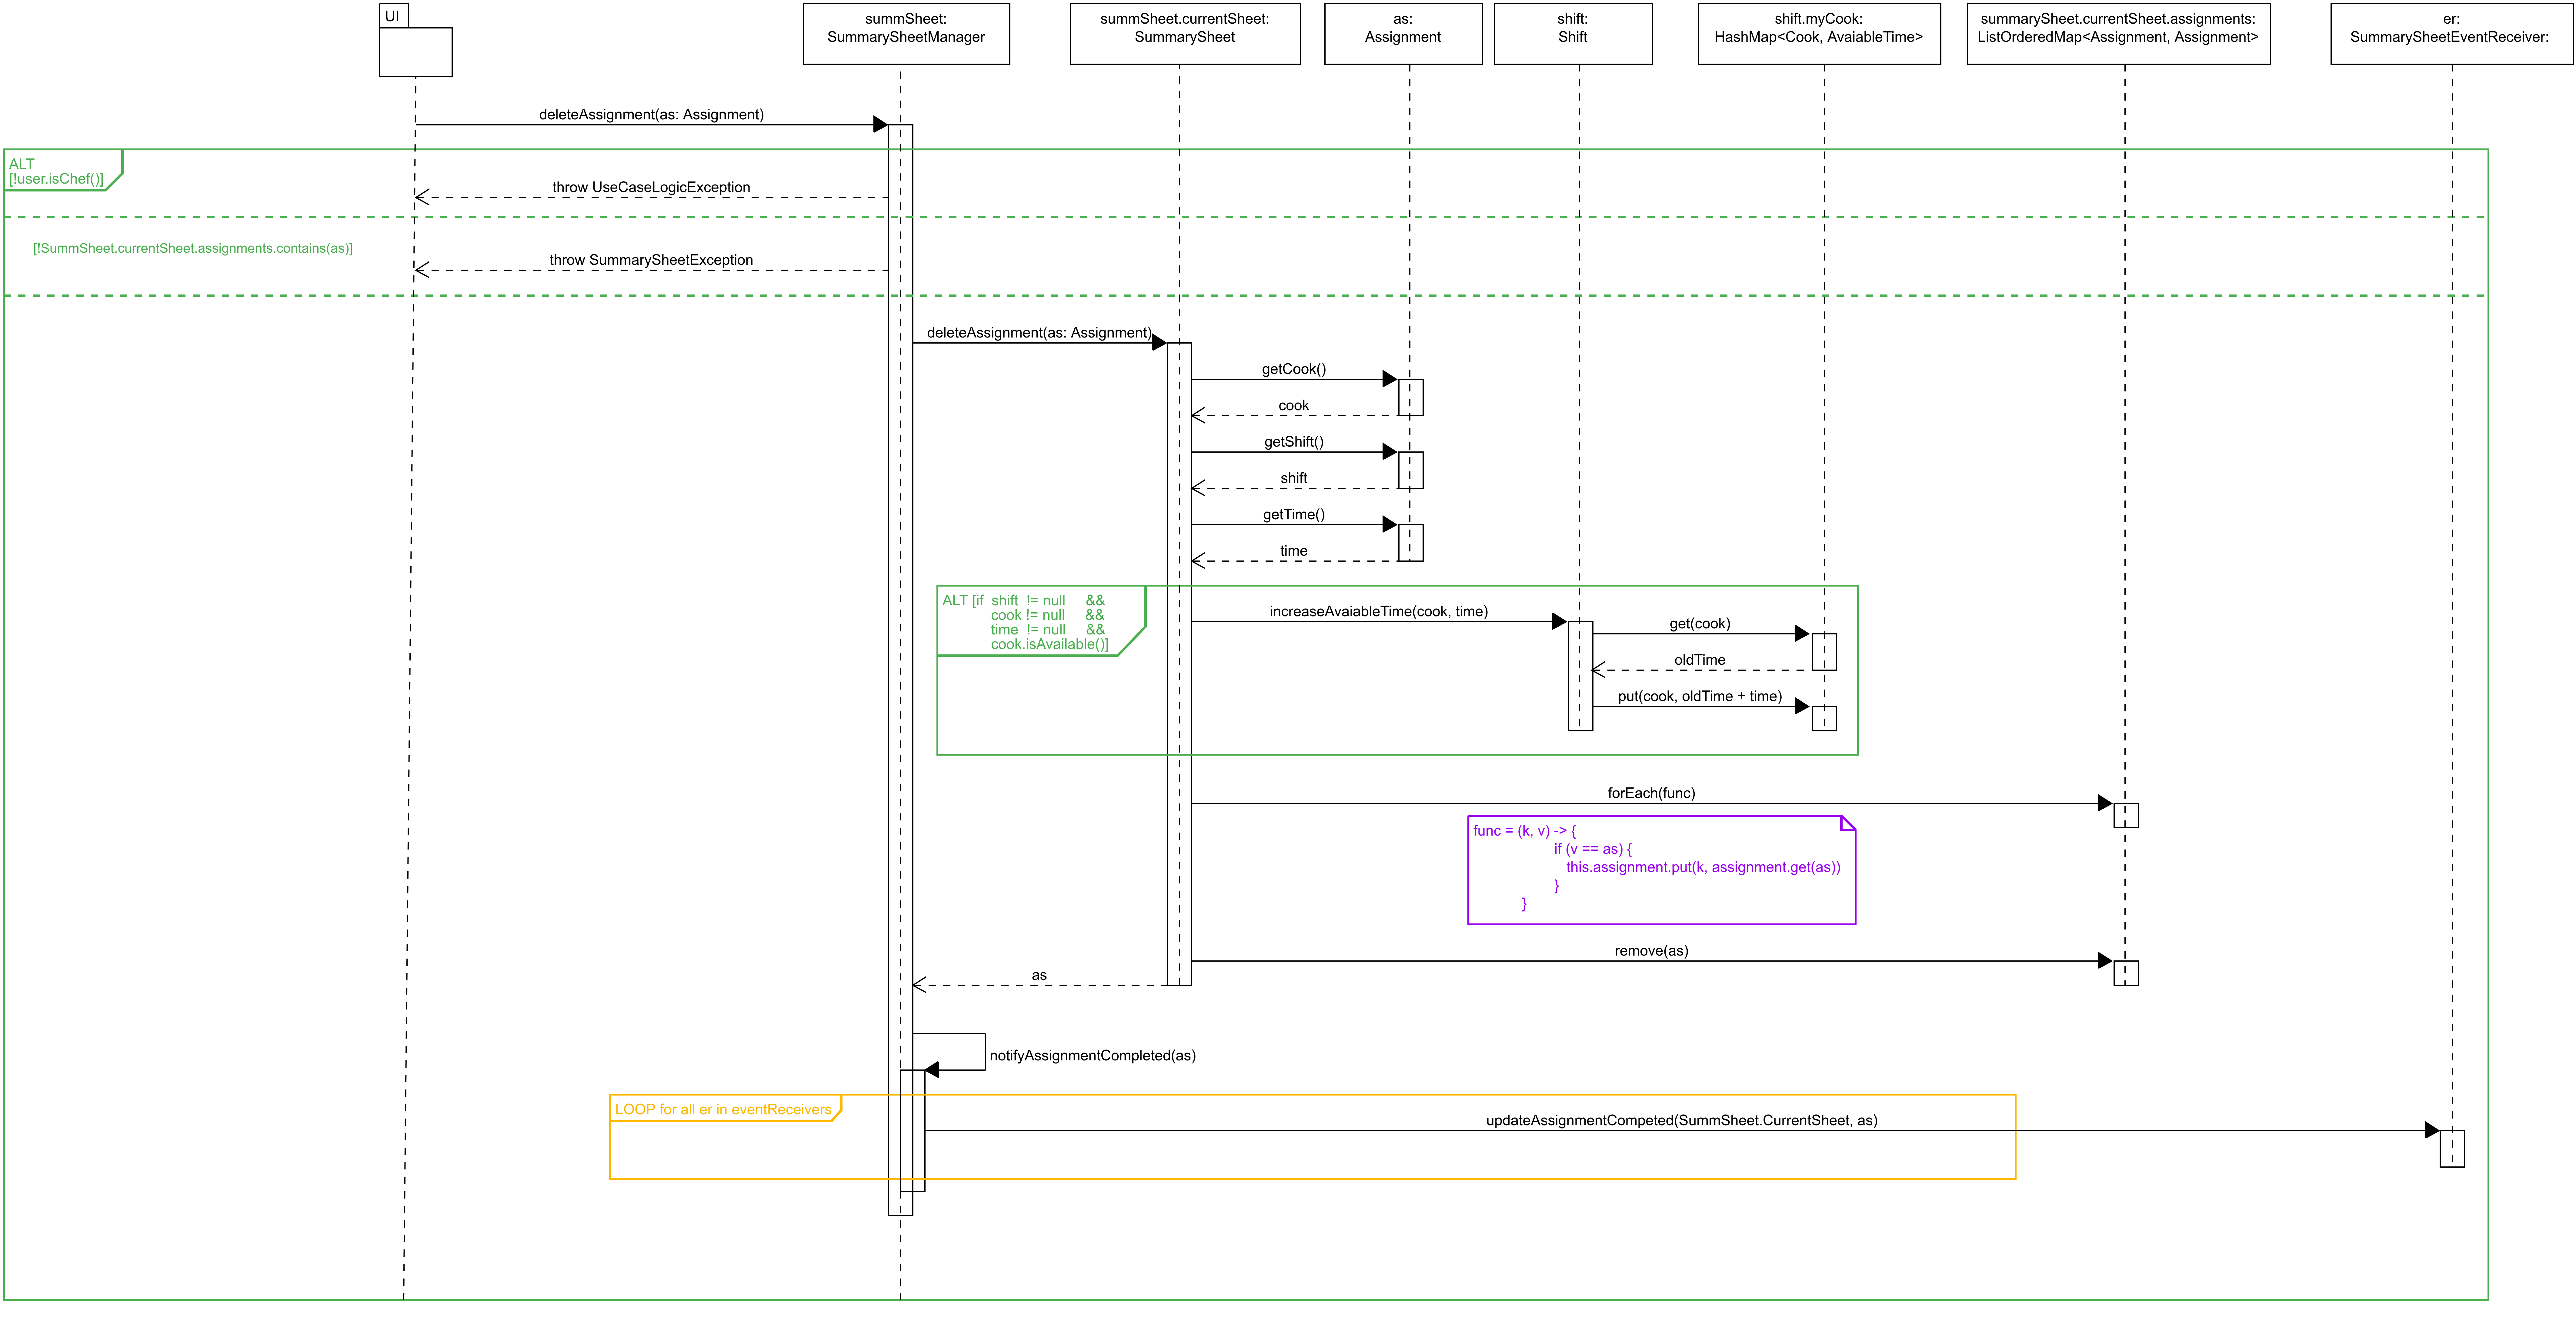
\includegraphics[max width=\textwidth, max height=190mm]{../resources/img/GCC/DSD/op5b.png}